\chapter{RNN for session-based recommendation}
In this chapter we explain the work we did on implementing a RNN for session-based recommendations. We used the Tensorflow \cite{tensorflow2015-whitepaper} library, and our code is available here \cite{skrede:code}.

\section{Goal}
From the papers we have looked at in Chapter \ref{chp:sota}, it is clear that a RNN can perform really well as a session-based recommender. It is also clear that there are possibilities to improve performance through different techniques and architectures. To be able to do our own experimentation and exploration in the domain we needed to implement a model of our own. We decided to use Tensorflow to implement a model heavily inspired by the model by Hidasi et al. in \cite{DBLP:journals/corr/HidasiKBT15}. This would allow us to familiarize ourselves with the software library and give us a model that could be used for further experimentation. We wanted our model to achieve similar performance to the one created by Hidasi et al.

\section{Implementation}
We have described the model created by Hidasi et al. in Section \ref{sec:hidasi-sess-based-rnn} and in Figure \ref{fig:gru4rec-network}. They used Theano for their implementation, the code is available at GitHub \cite{hidasi:code}. In this section we describe our implementation. Since our model is similar to the one by Hidasi et al., the reader is referred to \ref{sec:hidasi-sess-based-rnn} for more details. Here we focus on differences between the two models, and only briefly describe the similar parts. Our model is illustrated in Figure \ref{fig:skrede-rnn}

\begin{figure}[htp]
	\centering
	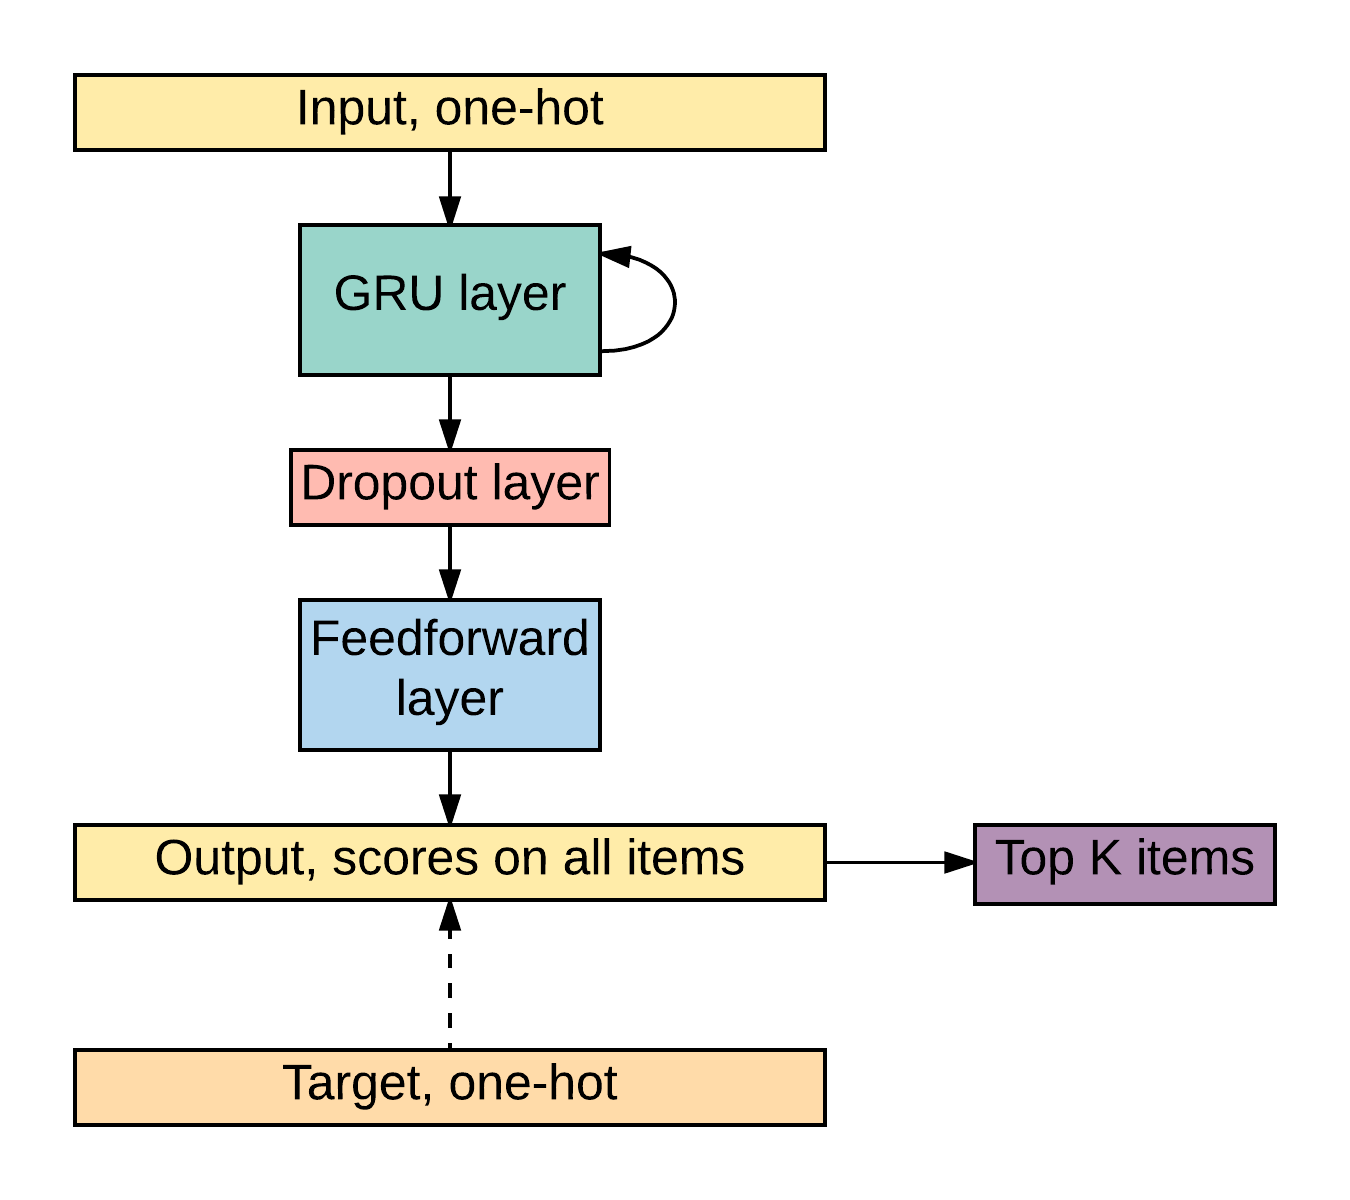
\includegraphics[width=1.0\textwidth]{fig/skrede-rnn.png}
	\caption{Illustration of the model we implemented, inspired by the model from \cite{DBLP:journals/corr/HidasiKBT15}.}
	\label{fig:skrede-rnn}
\end{figure}

The input is a one-hot representation of the clicked item in each sequence, which is sent into a GRU layer with 100 units. Between each sequence, the hidden state of the GRU layer is reset. Dropout is applied to the output from the GRU layer, with a dropout rate of 50\%. Dropout is not applied during testing. Then the output is sent through a feedforward layer and outputs scores for all items. Softmax cross-entropy is used on the output, with the one-hot representation of the next click as the label, to compute the loss. Adam \cite{DBLP:journals/corr/KingmaB14} is used for training, with a learning rate of 0.001. During testing, the indexes of the top K scores are retrieved as the models predictions.

Some of our choices and parameters are chosen somewhat random based on what we know worked well in similar models. We wanted to test with different parameters and solutions to optimize our model, unfortunately we were stuck for a long time, trying to get the model to run at a feasible speed. Thus, some of the parameters can probably be optimized.

Cross-entropy for calculating loss was chosen because Tensorflow already has support for it. We added dropout as we wanted to see what effect it would have on performance (both accuracy and runtime). All sequences were padded to the same length, for example length 10. This was because Tensorflow requires it. The padded clicks are outputted as all-zero vectors from the GRU layer. We wanted to experiment with adding bias in the feedforward layer, but because we only recently were able to use masking to ignore the padded all-zero vectors, bias has not been used. The problem is that the bias would have been applied to the padded vectors, which would affect training. Training was done in mini-batches of size 200, and the examples in each mini-batch were sampled randomly from the dataset.

We tested the effect of using a feedforward layer by comparing the model with and without that layer. We only tested this on our smallest dataset, but the model was both faster and more accurate when a feedforward layer was used. 
%explain the paper what i have tried to implement
%what did i want to achieve 
%core of what i implemented